\documentclass[conference]{IEEEtran}
\usepackage{cite}
\usepackage{amsmath}
\usepackage{graphicx}
\usepackage{url}
\usepackage{booktabs}
\usepackage[utf8]{inputenc}

% Layout tightening within IEEE conference style
\setlength{\textfloatsep}{3pt plus 1pt minus 1pt}
\setlength{\intextsep}{3pt plus 1pt minus 1pt}
\setlength{\abovecaptionskip}{1pt}
\setlength{\belowcaptionskip}{0pt}
\setlength{\dbltextfloatsep}{3pt plus 1pt minus 1pt}
\linespread{0.96}

\begin{document}

\title{\large Caption-Guided Cross-Attention Fusion for Remote Sensing\\Land-Cover Classification and Segmentation}

\author{\IEEEauthorblockN{Süleyman Ceran}
\IEEEauthorblockA{Middle East Technical University\\
Graduate School of Informatics\\
DI 725 -- Transformers and Attention-Based Deep Networks}}

\maketitle

\begin{abstract}
We compare four cross-modal fusion strategies for caption-guided remote sensing scene understanding on a 10{,}024-image subset of ARAS400K. A frozen RemoteCLIP-ViT-B/32 backbone is paired with late, FiLM, gated, and cross-attention (CA) fusion modules over five LLM-generated caption types, and the same modules are applied to patch-level multi-label classification and segmentation. CA wins every head-to-head against late fusion across captions, seeds, and tasks, reaching mAP $0.948 \pm 0.003$ and mIoU $0.711 \pm 0.003$. Gated fusion underperforms late concatenation in both tasks, a negative result we report. We further conduct three ablations. A threshold sensitivity sweep ($\tau \in \{5, 10, 20\}\%$) shows the fusion gain over the image-only baseline grows monotonically with $\tau$, from $+0.097$ to $+0.153$ mAP. A full $5 \times 4$ segmentation matrix confirms the fusion ranking at scale. A backbone-capacity ablation to RemoteCLIP-ViT-L/14 decreases segmentation mIoU by $0.041$, exposing a frozen-backbone limit that motivates parameter-efficient fine-tuning as future work. All 500+ training runs and code are public.
\end{abstract}

% =============================================================================
\section{Introduction}

Remote sensing (RS) imagery contains heterogeneous land cover at many spatial scales. Recent vision-language models (VLMs) generate captions that describe each scene in natural language, raising a practical question: can captions improve scene-level prediction beyond what an image-only model achieves? The answer depends on how the modalities are fused.

We study this question on a 10{,}024-image subset of ARAS400K~\cite{caglar2026aras400k} (the validation subset of the released $400{,}240$-image corpus, comprising $100{,}240$ real and $300{,}000$ synthetic images), with 7-class segmentation masks, composition percentages, and five LLM-generated caption strategies (vision-only, text-only from composition, and hybrid). Captions for the same image can range from highly leaky (the hybrid and text-only streams encode composition percentages literally and these percentages also define our multi-label targets) to noisy and unreliable (vision-only LLM captions hallucinate on this subset, for example labelling a 92\%-grass scene as ``barren''). This spectrum tests how each fusion mechanism handles caption quality.

\textbf{Research question:} How effective is cross-attention multi-modal fusion compared to late fusion for RS scene understanding using ViTs and LLM-generated captions?

\textbf{Contributions:} (i) A four-way fusion comparison (late, FiLM, gated, CA) with three seeds across 5 captions and 2 tasks. (ii) A negative result: gated fusion underperforms late concatenation, the sigmoid gate collapses one modality. (iii) Three ablations: threshold sensitivity, a full $5 \times 4$ segmentation matrix, and a backbone-capacity ablation that severely affects segmentation results in an unexpected direction. (iv) An example-samples figure that makes the inputs and outputs concrete on three diverse validation scenes. (v) Public code, 500+ tracked runs, and reproducible feature caches.

% =============================================================================
\section{Literature Survey}

VLMs jointly represent visual and textual information through contrastive learning~\cite{radford2021clip} and have gained traction in RS, where Wen et al.~\cite{wen2024vlm} identify cross-modal fusion as a major open challenge. RemoteCLIP~\cite{liu2024remoteclip}, the first CLIP adapted to RS, outperforms vanilla CLIP by up to 6.39\% on zero-shot classification via domain-adapted pretraining. Multimodal LLMs such as EarthGPT~\cite{zhang2024earthgpt} and RingMoGPT~\cite{wang2025ringmogpt} unify captioning, VQA, grounding, and change detection within a single instruction-tuned framework.

A central design choice is how to fuse the two modalities. Cross-modal attention has beaten unimodal methods on RS VQA~\cite{bazi2022bimodal} and visual grounding~\cite{lan2024grounding}, while SegCLIP~\cite{zhang2024segclip} fuses text with image features for RS segmentation. FiLM~\cite{perez2018film} offers an attention-free alternative through per-feature affine modulation. Few studies directly compare these mechanisms on RS scene-level tasks, and the role of caption-generation strategy on fusion performance remains under-explored despite evidence that caption source and quality matter~\cite{chen2024sharegpt4v}.

% =============================================================================
\section{Methods}

\textbf{Task:} An obvious formulation of the problem is 8-way dominant-cover classification at a 50\% threshold (7 land-cover classes plus an eighth ``no dominant'' class for scenes where no class exceeds the threshold). This formulation turns out to be trivial under text input alone (mAP $\approx 0.83$ from captions). We instead use 7-bit multi-label class presence at threshold $\tau$, with $\tau = 10\%$ as the default. The same image patch features drive a per-patch segmentation head on a $7 \times 7$ grid (Path~B).

\textbf{Backbone:} We use a frozen RemoteCLIP-ViT-B/32 backbone~\cite{liu2024remoteclip}. Per-token features are captured through forward hooks on the visual \texttt{ln\_post} and text \texttt{ln\_final} layers, after which we apply the model's own projection per token. This gives 50 image tokens (CLS + 49 patches) and 77 text tokens at 512 dim.

\textbf{Fusion modules:} Four variants share a 256-unit ReLU--Dropout--Linear head. Late concatenates pooled image and text vectors. FiLM generates per-feature $(\gamma, \beta)$ from pooled text and modulates the image CLS, with the modulator's final layer zero-initialised so the model starts at the image-only baseline. Gated mixes the two pooled vectors through a sigmoid gate. Cross-Attention uses \texttt{nn.MultiheadAttention} with 8 heads. For classification, text tokens are queries over image patches as keys and values, mean-pooled before the head. For segmentation the direction is inverted: image patches are queries over text tokens as keys and values, producing per-patch logits. Only the fusion module and head are trained.

\begin{figure*}[t]
\centering
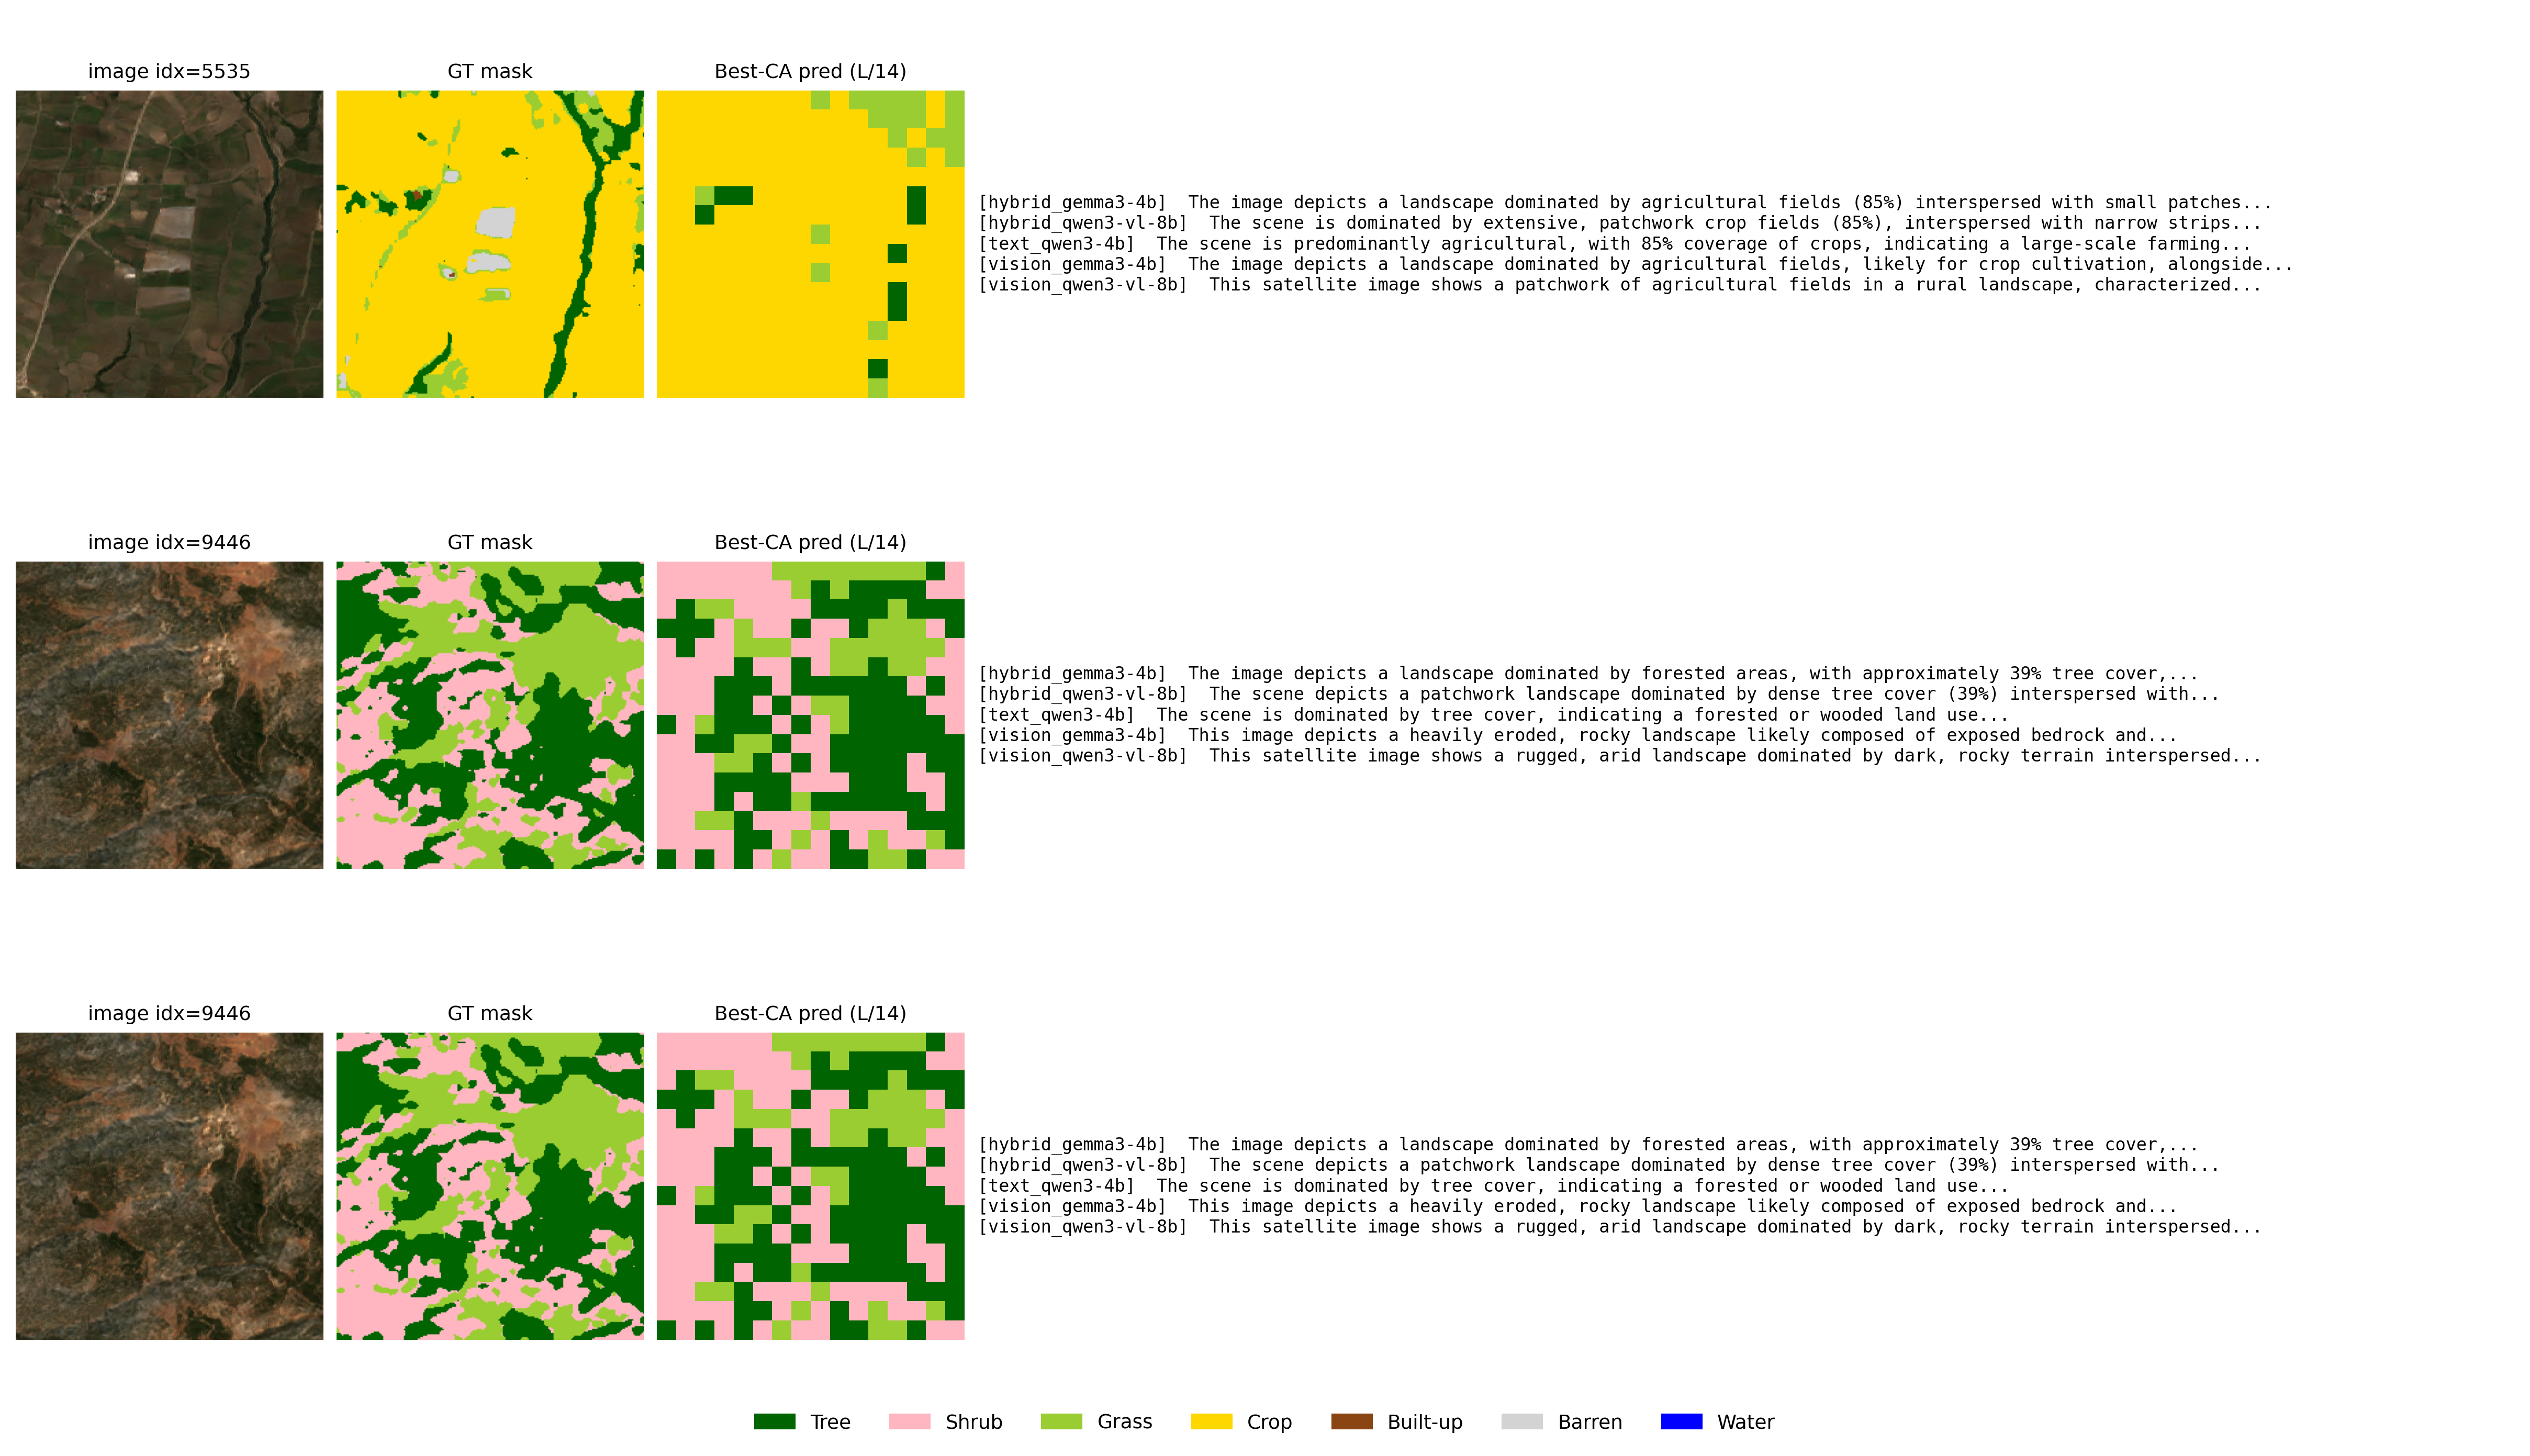
\includegraphics[width=0.92\textwidth]{figures/fig_example_samples.png}
\caption{\footnotesize Representative validation scenes. Each row shows the input image, ground-truth mask, best-CA segmentation prediction, and the five LLM caption strategies (truncated). Predictions are shown at the L/14 backbone because the $16 \times 16$ patch grid is visually finer than the $7 \times 7$ B/32 grid. Quantitative results elsewhere use B/32 as the main setting. Top, a dominant-class scene (Crop $85\%$). Middle, a balanced multi-class scene (Tree, Shrub, Grass each $\geq 28\%$). Bottom, a forested scene with a notable minor-class component (Shrub $19\%$).}
\label{fig:examples}
\end{figure*}

\textbf{Training and evaluation:} All conditions use the full 10{,}024-image subset with an 80/20 stratified split on dominant class. Each run uses AdamW (lr~$10^{-3}$, weight-decay~$10^{-4}$, 30 epochs, batch 256 for Path~A and 128 for Path~B) with three random seeds. Metrics are mAP and per-class F1 (Path~A) and mIoU and per-class IoU (Path~B). With features cached after a single backbone pass, the entire experimental matrix ($\approx 500$ runs, broken down as 117 main + 189 threshold + 63 full B/32 seg + 126 L/14) completes in $\approx 3$ hours on one A100. All runs are public on Weights \& Biases and the codebase is on GitHub~\cite{repo2026,wandb2026}.

% =============================================================================
\section{Results}

\subsection{Main results on the B/32 backbone}

\textbf{Path~A classification:} The best run is cross-attention with \texttt{hybrid\_qwen3-vl-8b} at mAP $0.948 \pm 0.003$ versus an image-only baseline of $0.817 \pm 0.001$ (Fig.~\ref{fig:heatmap}, Table~\ref{tab:pathA}). CA beats late fusion on every caption ($\Delta$ mAP from $+0.036$ to $+0.051$). FiLM is the close runner-up at $0.005$ mAP behind CA. Gated fusion underperforms even simple late concatenation, plausibly because the sigmoid gate collapses toward a near-unimodal representation, although direct inspection of gate values would be needed to confirm this.

\begin{figure}[t]
\centering
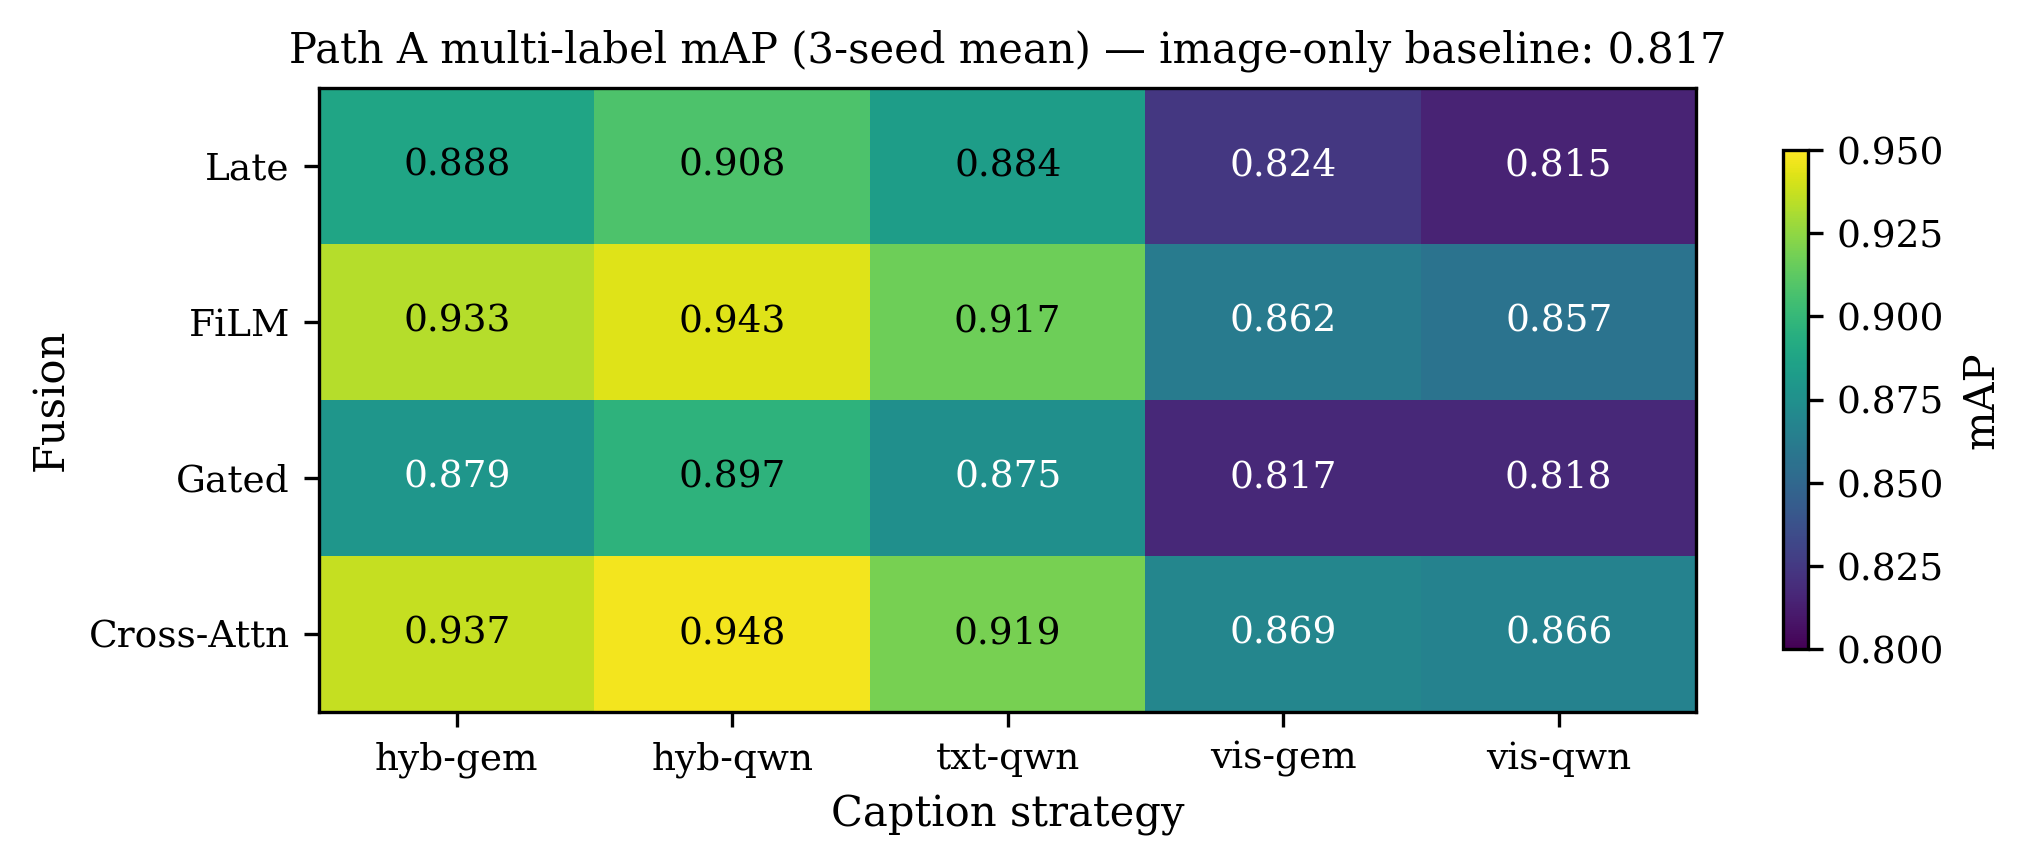
\includegraphics[width=\columnwidth]{figures/fig1_fusion_heatmap.png}
\caption{\footnotesize Path~A multi-label mAP at $\tau = 10\%$ (3-seed mean). Rows are fusion modules, columns are caption strategies. Image-only baseline: $0.817 \pm 0.001$.}
\label{fig:heatmap}
\end{figure}

\textbf{Noise robustness:} With the noisy \texttt{vision\_qwen3-vl-8b} caption, late fusion gains nothing over image-only ($0.815 \approx 0.817$) while CA recovers $+0.049$ mAP. The pattern is consistent with CA being more robust to noisy captions than the parametric fusions, although token-level attention analysis would be needed to confirm whether unreliable tokens are explicitly down-weighted.

\textbf{Per-class decomposition:} Minor classes that the image-only baseline fails on (Shrub F1 $0.00$, Built-up $0.65$, Barren $0.61$) recover under CA (Shrub $0.66$, Built-up $0.79$, Barren $0.79$). Captions and images carry complementary information on these classes.

\begin{table}[t]
\centering
\caption{\footnotesize Path~A best result per fusion family (3-seed mean, $\tau = 10\%$, B/32 backbone).}
\label{tab:pathA}
\footnotesize
\setlength{\tabcolsep}{4pt}
\renewcommand{\arraystretch}{0.95}
\begin{tabular}{lccc}
\toprule
Fusion & Best mAP & Macro F1 & Mean mAP \\
\midrule
Image-only           & $0.817 \pm 0.001$ & $0.702 \pm 0.006$ & ---     \\
Late                 & $0.908 \pm 0.003$ & $0.836 \pm 0.009$ & $0.864$ \\
Gated                & $0.897 \pm 0.001$ & $0.811 \pm 0.007$ & $0.857$ \\
FiLM                 & $0.943 \pm 0.001$ & $0.876 \pm 0.008$ & $0.903$ \\
Cross-Attn  & $0.948 \pm 0.003$ & $0.867 \pm 0.014$ & $0.908$ \\
\bottomrule
\end{tabular}
\end{table}

\textbf{Path~B segmentation:} On the full $5 \times 4$ B/32 matrix (Table~\ref{tab:pathB}), the best run is CA + \texttt{hybrid\_qwen3-vl-8b} at mIoU $0.711 \pm 0.003$ versus image-only $0.574 \pm 0.003$. The Path~A fusion ranking transfers exactly. The CA-vs-Late delta is positive on all five captions, the noise-robustness signature persists with vision-only captions, and per-class IoU lifts concentrate on minor classes (Shrub $0.05 \to 0.41$, Barren $0.39 \to 0.59$).

\begin{table}[t]
\centering
\caption{\footnotesize Path~B segmentation mIoU per fusion family across the five caption strategies (3-seed mean, B/32 backbone, $7 \times 7$ patch grid). Image-only baseline mIoU $0.574 \pm 0.003$. Best per row in bold.}
\label{tab:pathB}
\footnotesize
\setlength{\tabcolsep}{3pt}
\renewcommand{\arraystretch}{0.95}
\begin{tabular}{lcccccc}
\toprule
Fusion & hyb-gem & hyb-qwn & txt-qwn & vis-gem & vis-qwn & Mean \\
\midrule
Late                  & $0.663$ & $0.669$ & $0.673$ & $0.582$ & $0.575$ & $0.632$ \\
Gated                 & $0.660$ & $0.667$ & $0.675$ & $0.581$ & $0.573$ & $0.631$ \\
FiLM                  & $0.689$ & $0.694$ & $0.693$ & $0.615$ & $0.613$ & $0.661$ \\
Cross-Attn   & $0.709$ & $0.711$ & $0.701$ & $0.608$ & $0.610$ & $0.668$ \\
\bottomrule
\end{tabular}
\end{table}

\subsection{Ablation study}

Three ablations probe distinct dimensions of the research question: task definition (threshold), task scope (full segmentation matrix), and backbone capacity (B/32 versus L/14).

\textbf{(A) Threshold sensitivity:} We sweep $\tau \in \{5, 10, 20\}\%$ over the full $5 \times 4$ Path~A matrix with 3 seeds (189 runs). The image-only baseline degrades as $\tau$ rises (mAP $0.841 \to 0.817 \to 0.791$) because higher thresholds drop minor positives. The CA-vs-baseline gap grows with $\tau$: $+0.097$ at $\tau = 5\%$, $+0.131$ at $\tau = 10\%$, and $+0.153$ at $\tau = 20\%$. Fig.~\ref{fig:tau} shows the family-wise best mAP per $\tau$. CA is best on average at every threshold. FiLM slightly exceeds CA at $\tau = 5\%$ ($0.944$ vs $0.938$) but trails at $\tau = 10\%$ and $\tau = 20\%$. The default $\tau = 10\%$ is a balanced operating point and does not change the fusion ranking.

\begin{figure}[t]
\centering
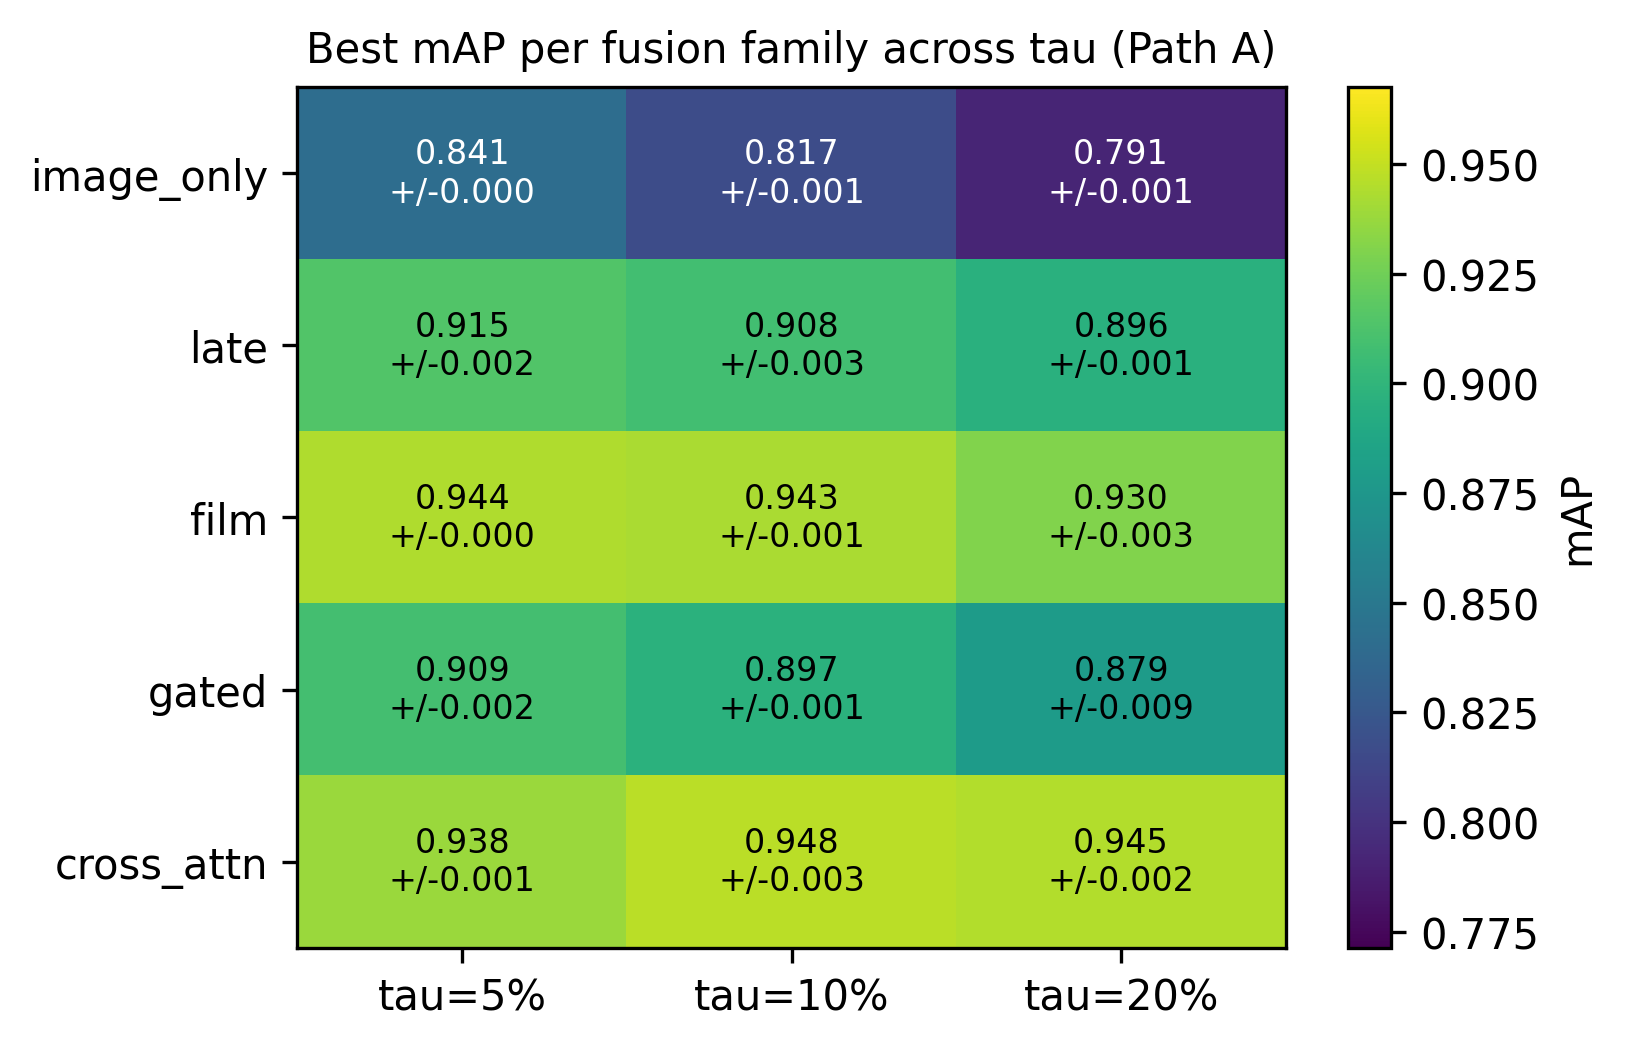
\includegraphics[width=\columnwidth]{figures/fig_tau_sensitivity.png}
\caption{\footnotesize Threshold ablation. Best mAP per fusion family at $\tau \in \{5, 10, 20\}\%$ on Path~A. Fusion gain over image-only is monotone in $\tau$.}
\label{fig:tau}
\end{figure}

\textbf{(B) Full segmentation matrix:} A preliminary segmentation run covered only 7 conditions (3 captions, late and CA). We close the matrix to all 21 conditions ($5 \times 4$ + image-only) with 3 seeds. The full matrix confirms the Path~A ranking transfers to dense prediction without exception: CA wins on each of the 5 captions, FiLM is the consistent runner-up, and gated again falls below late on average (mean mIoU $0.631$ vs $0.632$). This is the most direct test that the headline findings were not artefacts of the small condition set.

\textbf{(C) Backbone capacity (severely-affects ablation):} We re-extract patch features with a larger RemoteCLIP-ViT-L/14 backbone (304M params vs 86M, 16$\times$16 patches at 224 input vs 7$\times$7, feature dim 768 vs 512) and re-run both task matrices. The intent was to test whether higher patch resolution improves segmentation. Results contradict that hypothesis. On Path~A, L/14 only marginally improves the best CA mAP ($0.948 \to 0.956$) and degrades the image-only baseline ($0.817 \to 0.803$). On Path~B the effect is severe in the opposite direction: every fusion family loses mIoU under L/14, including the best CA run (mIoU $0.711 \to 0.670$, $\Delta = -0.041$). Fig.~\ref{fig:backbone} contrasts the two backbones per fusion family, and Table~\ref{tab:l14} reports per-class IoU at L/14. Despite the drop, the fusion ranking and per-class lift pattern of L/14 mirror those of B/32 (Shrub $0.034 \to 0.378$, $+0.344$, and Barren $0.310 \to 0.511$, $+0.200$). The pattern is preserved. Only the absolute scale shifts.

\begin{figure}[t]
\centering
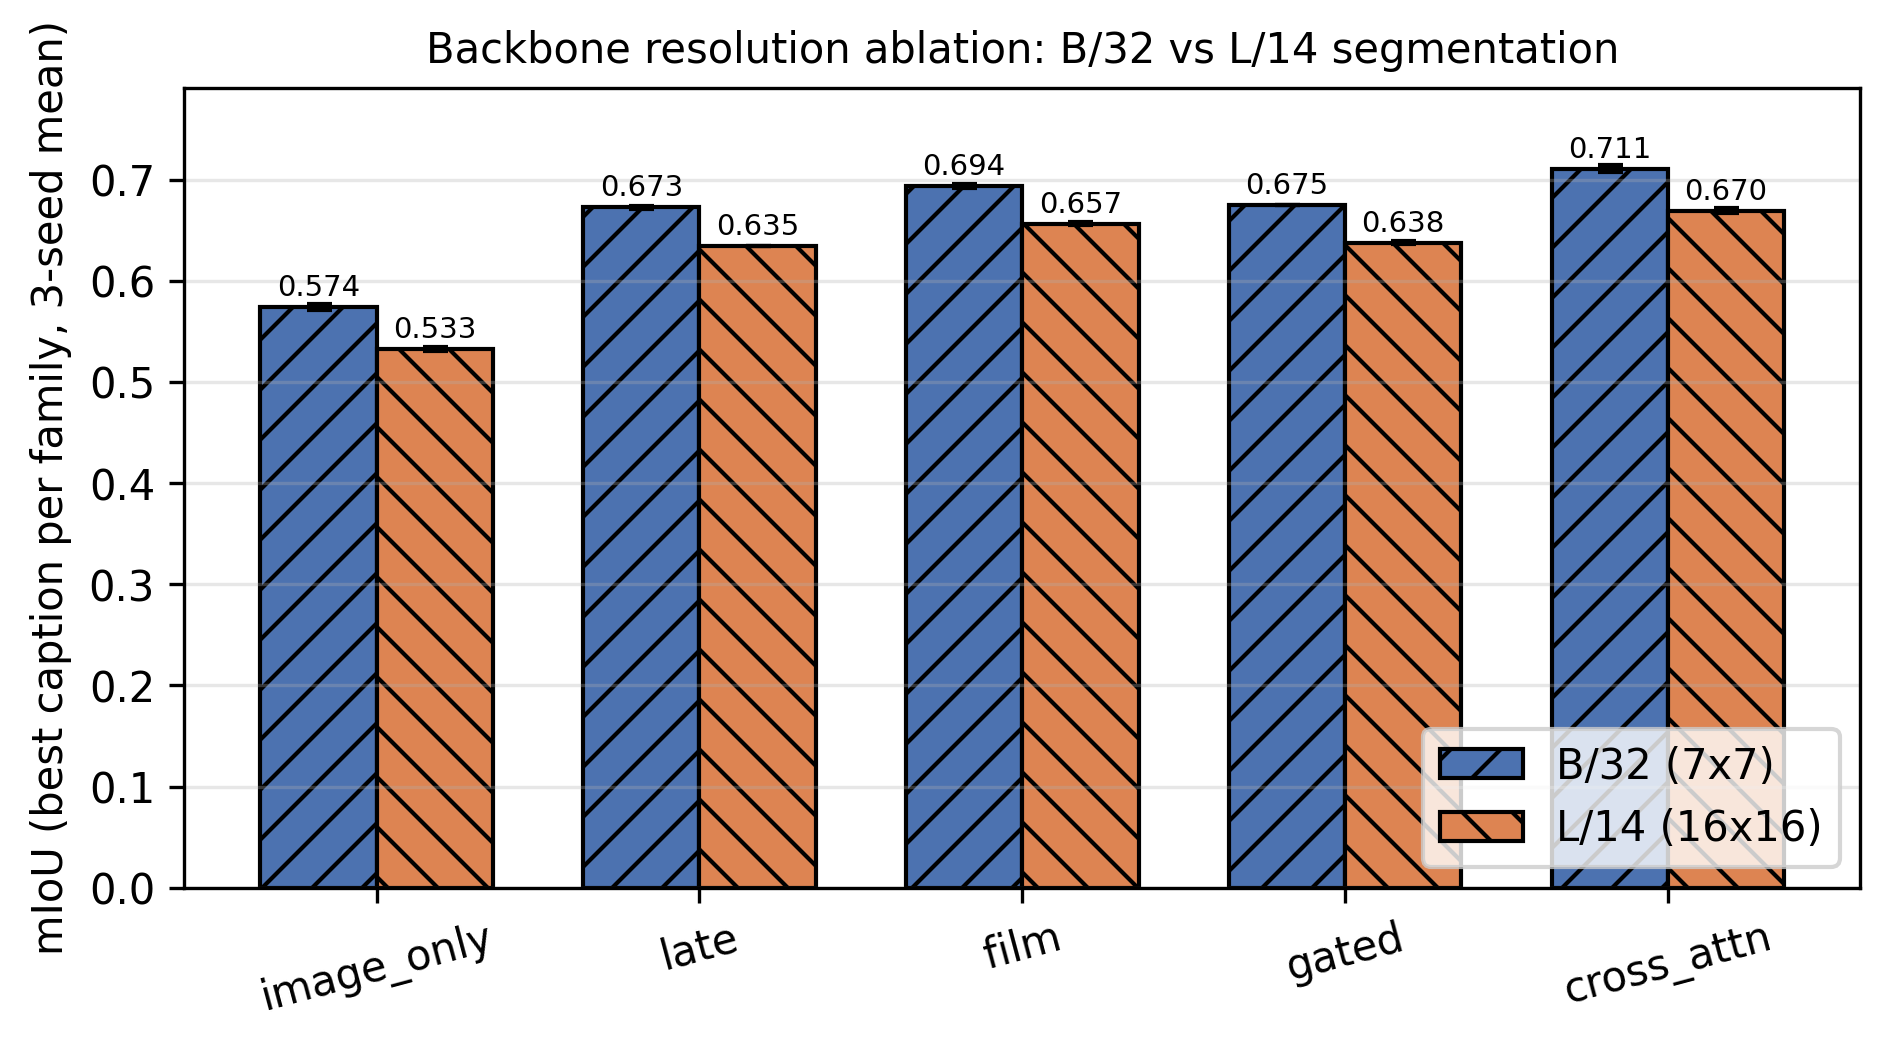
\includegraphics[width=\columnwidth]{figures/fig_l14_vs_b32_seg.png}
\caption{\footnotesize Backbone ablation. Best mIoU per fusion family at B/32 (hatch \texttt{//}) and L/14 (hatch $\backslash\backslash$). The larger, higher-resolution L/14 backbone reduces segmentation mIoU across all fusion families.}
\label{fig:backbone}
\end{figure}

\begin{table}[t]
\centering
\caption{\footnotesize Per-class IoU under the L/14 backbone, image-only versus best CA (\texttt{hybrid\_qwen}). Fusion-induced lift is largest on minor classes.}
\label{tab:l14}
\footnotesize
\setlength{\tabcolsep}{4pt}
\renewcommand{\arraystretch}{0.95}
\begin{tabular}{lccc}
\toprule
Class & Image-only & Best CA & $\Delta$ \\
\midrule
Tree     & $0.760$ & $0.814$ & $+0.054$ \\
Shrub    & $0.034$ & $0.378$ & $+0.344$ \\
Grass    & $0.715$ & $0.793$ & $+0.077$ \\
Crop     & $0.641$ & $0.759$ & $+0.118$ \\
Built-up & $0.505$ & $0.575$ & $+0.070$ \\
Barren   & $0.310$ & $0.511$ & $+0.200$ \\
Water    & $0.764$ & $0.858$ & $+0.094$ \\
\midrule
mIoU     & $0.533$ & $0.670$ & $+0.137$ \\
\bottomrule
\end{tabular}
\end{table}

% =============================================================================
\section{Discussion}

Across these experiments, CA consistently outperforms late fusion across captions, seeds, thresholds, and tasks. On the Path~A B/32 matrix the gain over the image-only baseline is $+0.131$ mAP. On the Path~B B/32 matrix it is $+0.137$ mIoU. On the L/14 backbone the absolute scale shifts but the relative gain is preserved (Path~B $+0.137$). The average family ranking is CA $\approx$ FiLM $>$ Late $\approx$ Gated, with CA giving the strongest main results and the most reliable improvement over late fusion. FiLM is competitive throughout and slightly exceeds CA in the $\tau{=}5\%$ setting ($0.944$ vs $0.938$ best mAP), so we do not claim that CA dominates FiLM unconditionally.

\textbf{Comparison with the literature:} Bazi et al.~\cite{bazi2022bimodal} report cross-attention beating unimodal methods on RS VQA, and Lan et al.~\cite{lan2024grounding} show the same on grounding. Our result is consistent with these findings on a third RS task type (scene-level multi-label classification) and on segmentation. SegCLIP~\cite{zhang2024segclip} addresses RS segmentation with a related text-conditioned design. We use it as methodological context rather than a numerical baseline, since its datasets, class taxonomies, supervision, and evaluation protocols differ from ours. The vanilla-CLIP versus RemoteCLIP gap (avg.\ $+0.031$ mAP for RemoteCLIP in an earlier backbone-source ablation we ran on the same matrix) is qualitatively consistent with the 6.39\% zero-shot gap reported by Liu et al.~\cite{liu2024remoteclip}, even though their evaluation protocol is different.

\textbf{Why does L/14 regress on segmentation?} The L/14 backbone has 3.5$\times$ more parameters and 5.2$\times$ more patch tokens, but the trainable head and the training budget are unchanged. More spatial tokens through the same cross-entropy loss make per-patch optimisation noisier, and the L/14 image embedding is trained for image-level alignment rather than patch-level discrimination. The image-only seg baseline already drops by $0.041$ before any fusion is added, supporting this reading. Partial fine-tuning, for instance LoRA on the last attention blocks, is a natural next experiment to test whether this gap can be recovered.

% =============================================================================
\section{Conclusion}

We compared four cross-modal fusion strategies for caption-guided RS land-cover classification and segmentation on a 10{,}024-image subset of ARAS400K with a frozen RemoteCLIP backbone. Cross-attention consistently outperformed late fusion across 5 captions, 3 seeds, two tasks, two backbones, and three thresholds, and gave the strongest main result (mAP $0.948 \pm 0.003$ on Path~A, mIoU $0.711 \pm 0.003$ on Path~B). FiLM was competitive throughout and slightly exceeded CA at $\tau{=}5\%$. Threshold sensitivity showed the fusion gain over the image-only baseline grows monotonically with $\tau$. The full segmentation matrix replicated the Path~A pattern at scale. A backbone-capacity ablation to ViT-L/14 produced a $0.041$ mIoU drop on segmentation, revealing a limit of the frozen-backbone paradigm. Because the hybrid and text-only captions are derived from the same composition statistics that define our multi-label targets, results in those settings should be read as oracle-text upper bounds rather than fully independent language supervision. The vision-only-caption results provide the cleaner test of caption-guided fusion. Parameter-efficient fine-tuning of the backbone is a natural future direction. The full codebase, $\approx 500$ tracked runs, and reproducible feature caches are public.

% =============================================================================
\scriptsize
\setlength{\IEEEilabelindent}{0pt}
\setlength{\IEEEiednormlabelsep}{0pt}
\renewcommand{\IEEEbibitemsep}{0pt plus 0.3pt}
\begin{thebibliography}{14}

\bibitem{radford2021clip}
A.~Radford \emph{et al.}, ``Learning transferable visual models from natural language supervision,'' \emph{ICML}, 2021.

\bibitem{wen2024vlm}
C.~Wen \emph{et al.}, ``Vision-Language Models in Remote Sensing,'' \emph{IEEE Geosci.\ Remote Sens.\ Mag.}, vol.~12, 2024.

\bibitem{liu2024remoteclip}
F.~Liu \emph{et al.}, ``RemoteCLIP: A Vision Language Foundation Model for Remote Sensing,'' \emph{IEEE TGRS}, vol.~62, 2024.

\bibitem{zhang2024earthgpt}
W.~Zhang \emph{et al.}, ``EarthGPT: A Universal Multimodal Large Language Model for Multisensor Image Comprehension in Remote Sensing,'' \emph{IEEE TGRS}, vol.~62, 2024.

\bibitem{wang2025ringmogpt}
P.~Wang \emph{et al.}, ``RingMoGPT: A Unified Remote Sensing Foundation Model for Vision, Language, and Grounded Tasks,'' \emph{IEEE TGRS}, vol.~63, 2025.

\bibitem{bazi2022bimodal}
Y.~Bazi \emph{et al.}, ``Bi-Modal Transformer-Based Approach for Visual Question Answering in Remote Sensing Imagery,'' \emph{IEEE TGRS}, vol.~60, 2022.

\bibitem{lan2024grounding}
M.~Lan \emph{et al.}, ``Language Query-Based Transformer for Visual Grounding on Remote Sensing Images,'' \emph{IEEE TGRS}, vol.~62, 2024.

\bibitem{zhang2024segclip}
S.~Zhang \emph{et al.}, ``SegCLIP: Multimodal Visual-Language and Prompt Learning for RS Semantic Segmentation,'' \emph{IEEE TGRS}, vol.~62, 2024.

\bibitem{perez2018film}
E.~Perez \emph{et al.}, ``FiLM: Visual reasoning with a general conditioning layer,'' \emph{AAAI}, 2018.

\bibitem{chen2024sharegpt4v}
L.~Chen \emph{et al.}, ``ShareGPT4V: Improving Large Multi-Modal Models with Better Captions,'' \emph{ECCV}, 2024.

\bibitem{caglar2026aras400k}
M.~Caglar, ``ARAS400K Remote Sensing Dataset,'' Zenodo, 2026, \url{https://zenodo.org/records/18890661}.

\bibitem{repo2026}
S.~Ceran, ``ARAS multi-modal attention land-cover classification,'' GitHub, 2026, \url{https://github.com/sceran/aras-multimodal-attention-landcover-classification}.

\bibitem{wandb2026}
S.~Ceran, ``DI~725 experiment tracking,'' Weights \& Biases, 2026.\ Projects: \url{https://wandb.ai/sceran/di725-phase2-main}, \url{https://wandb.ai/sceran/di725-phase2-backbone-vanilla}, \url{https://wandb.ai/sceran/di725-phase2-seg}, \url{https://wandb.ai/sceran/di725-phase3-tau}, \url{https://wandb.ai/sceran/di725-phase3-seg-full}, \url{https://wandb.ai/sceran/di725-phase3-l14-pathA}, \url{https://wandb.ai/sceran/di725-phase3-l14-seg}.

\end{thebibliography}

\end{document}
